\section{Testprotokoll: Burst}
\label{sec:Test:Burst}
Wie in Kapitel \ref{sec:TestUndNorm} erwähnt, werden Burst-Tests zurchgeführt. Zur Auswahl stehen gemäss Abbildung \ref{fig:BurstNorm} vier verschiedene Normprogramme. Es wurden alle Normprogramme durchgeführt, deren Ergebnisse werden nachfolgend dokumentiert. Der Testaufbau und die verwendeten Geräte werden in Kapitel \ref{sec:Testaufbau} erläutert.\\[0.5cm]
\begin{minipage}[b][10cm][t]{1\textwidth}
\centering
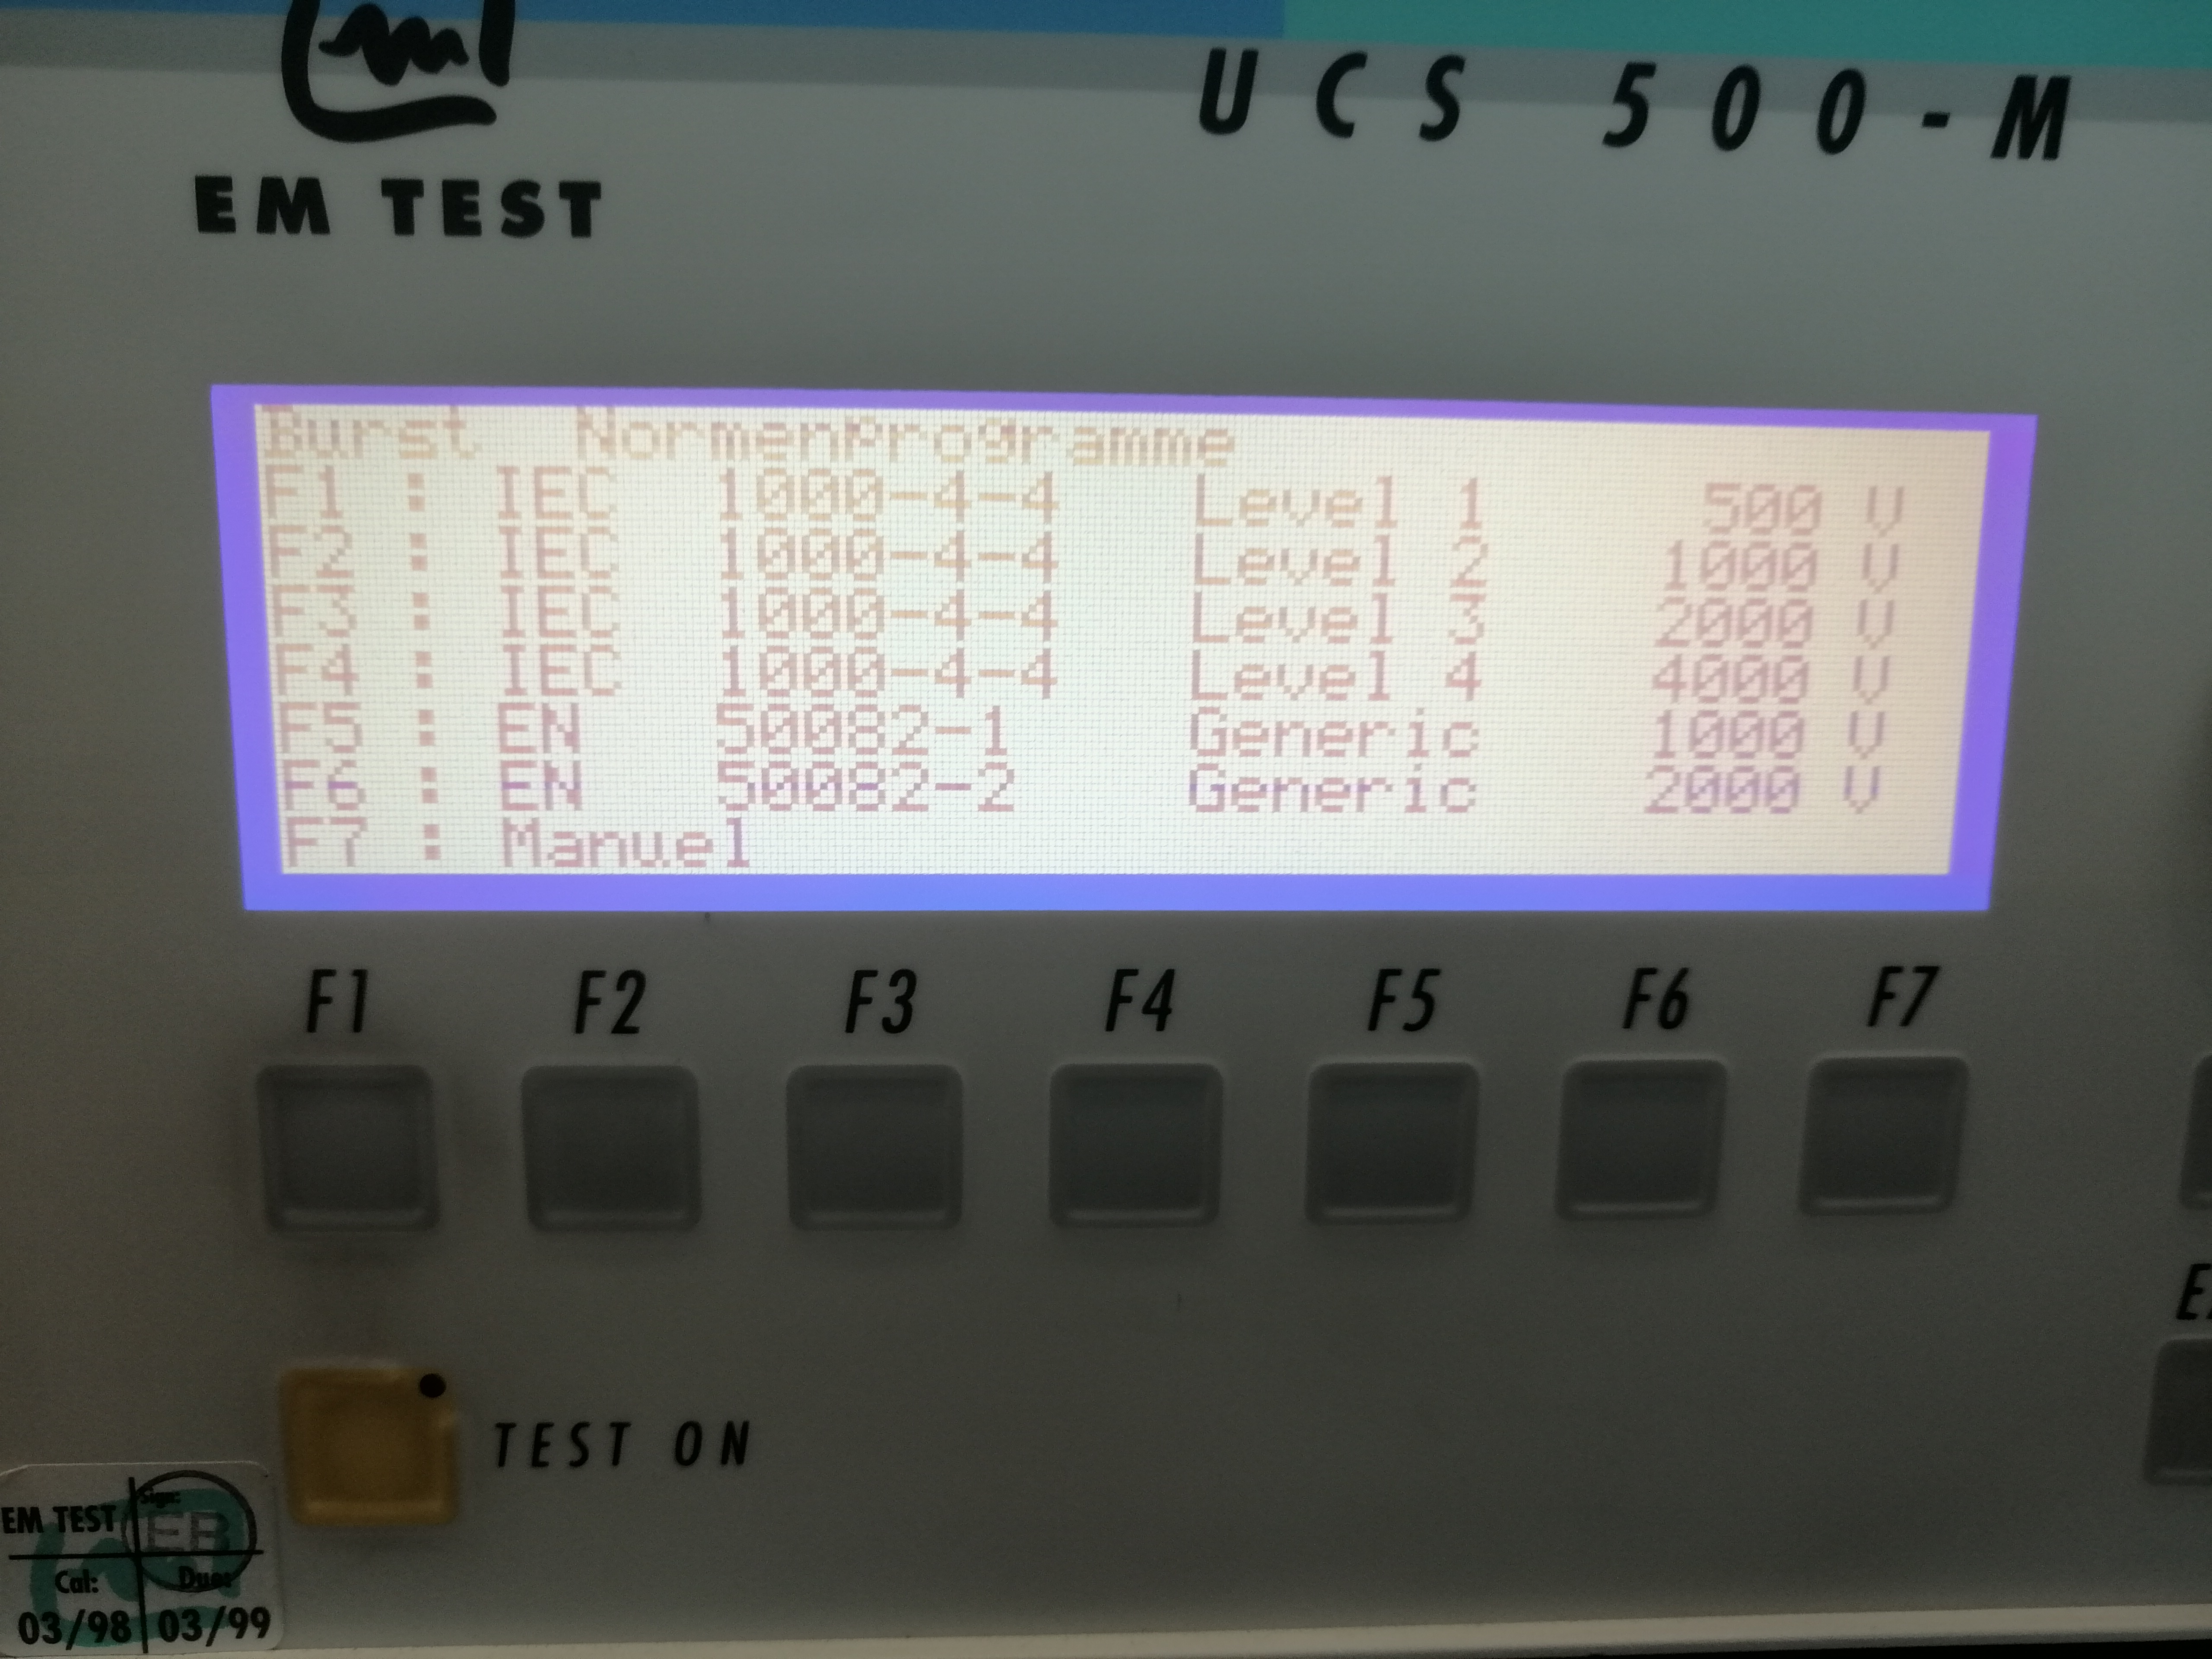
\includegraphics[angle=0,width=0.75\textwidth]{graphics/BurstNormprogramm.jpg}
\captionof{figure}{Auswahl der Normprogramme.}
\label{fig:BurstNorm}
\end{minipage}
Abbildung \ref{fig:BurstNorm} zeigt die verschiedenen Normprogramme, welche alle durchgeführt wurden.\\[0.25cm]
Die Auswirkungen der Tests wurden mit einem Oszilloskop gemessen. Die Messungen ergaben alle ein ähnliches Bild, weshalb der Einfachheit halber nur Bilder von einem Ergebnis gezeigt werden.\\[0.25cm]
\begin{minipage}[b][10cm][t]{1\textwidth}
\centering
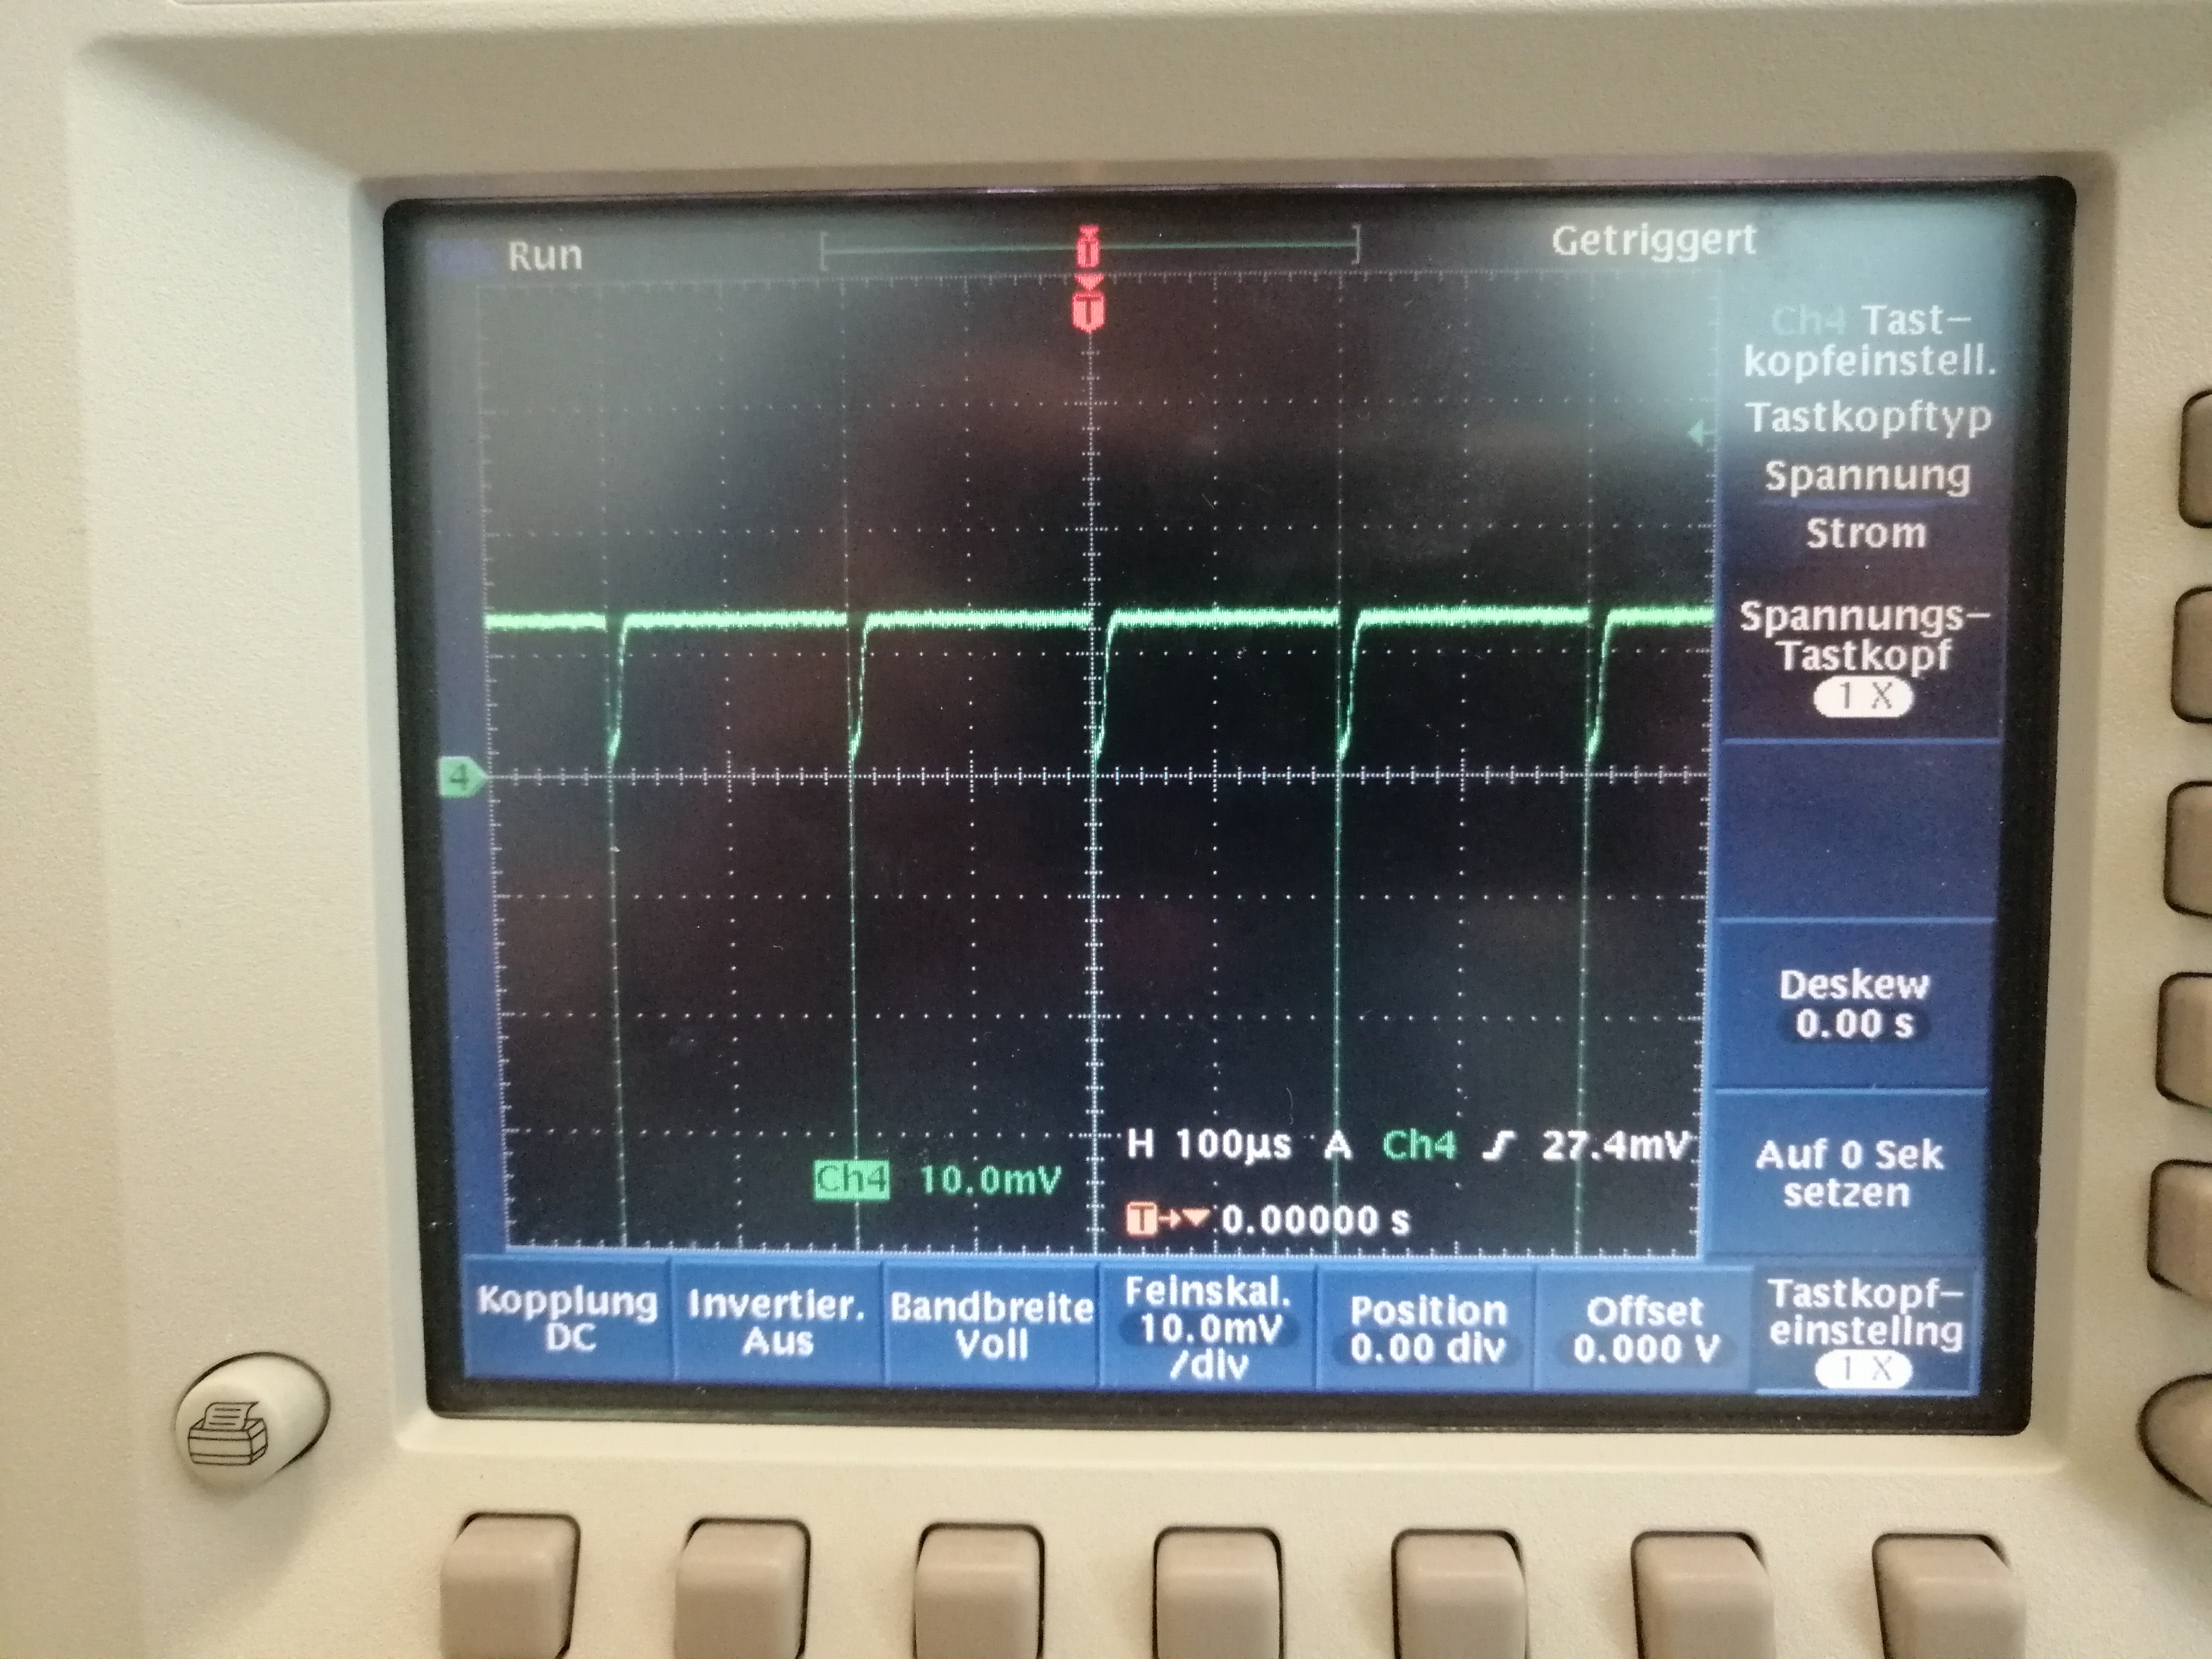
\includegraphics[angle=0,width=0.75\textwidth]{graphics/BurstE1.jpg}
\captionof{figure}{Signalmessung während Burst-Tests.}
\label{fig:BurstE1}
\end{minipage}
In Abbildung \ref{fig:BurstE1} ist zusehen, dass die Bursts das Signal zusammenreissen. Jedoch erholt sich das System schnell wieder nach ca 20$\mu s$.\\
[0.5cm]
\begin{minipage}[b][10cm][t]{1\textwidth}
\centering
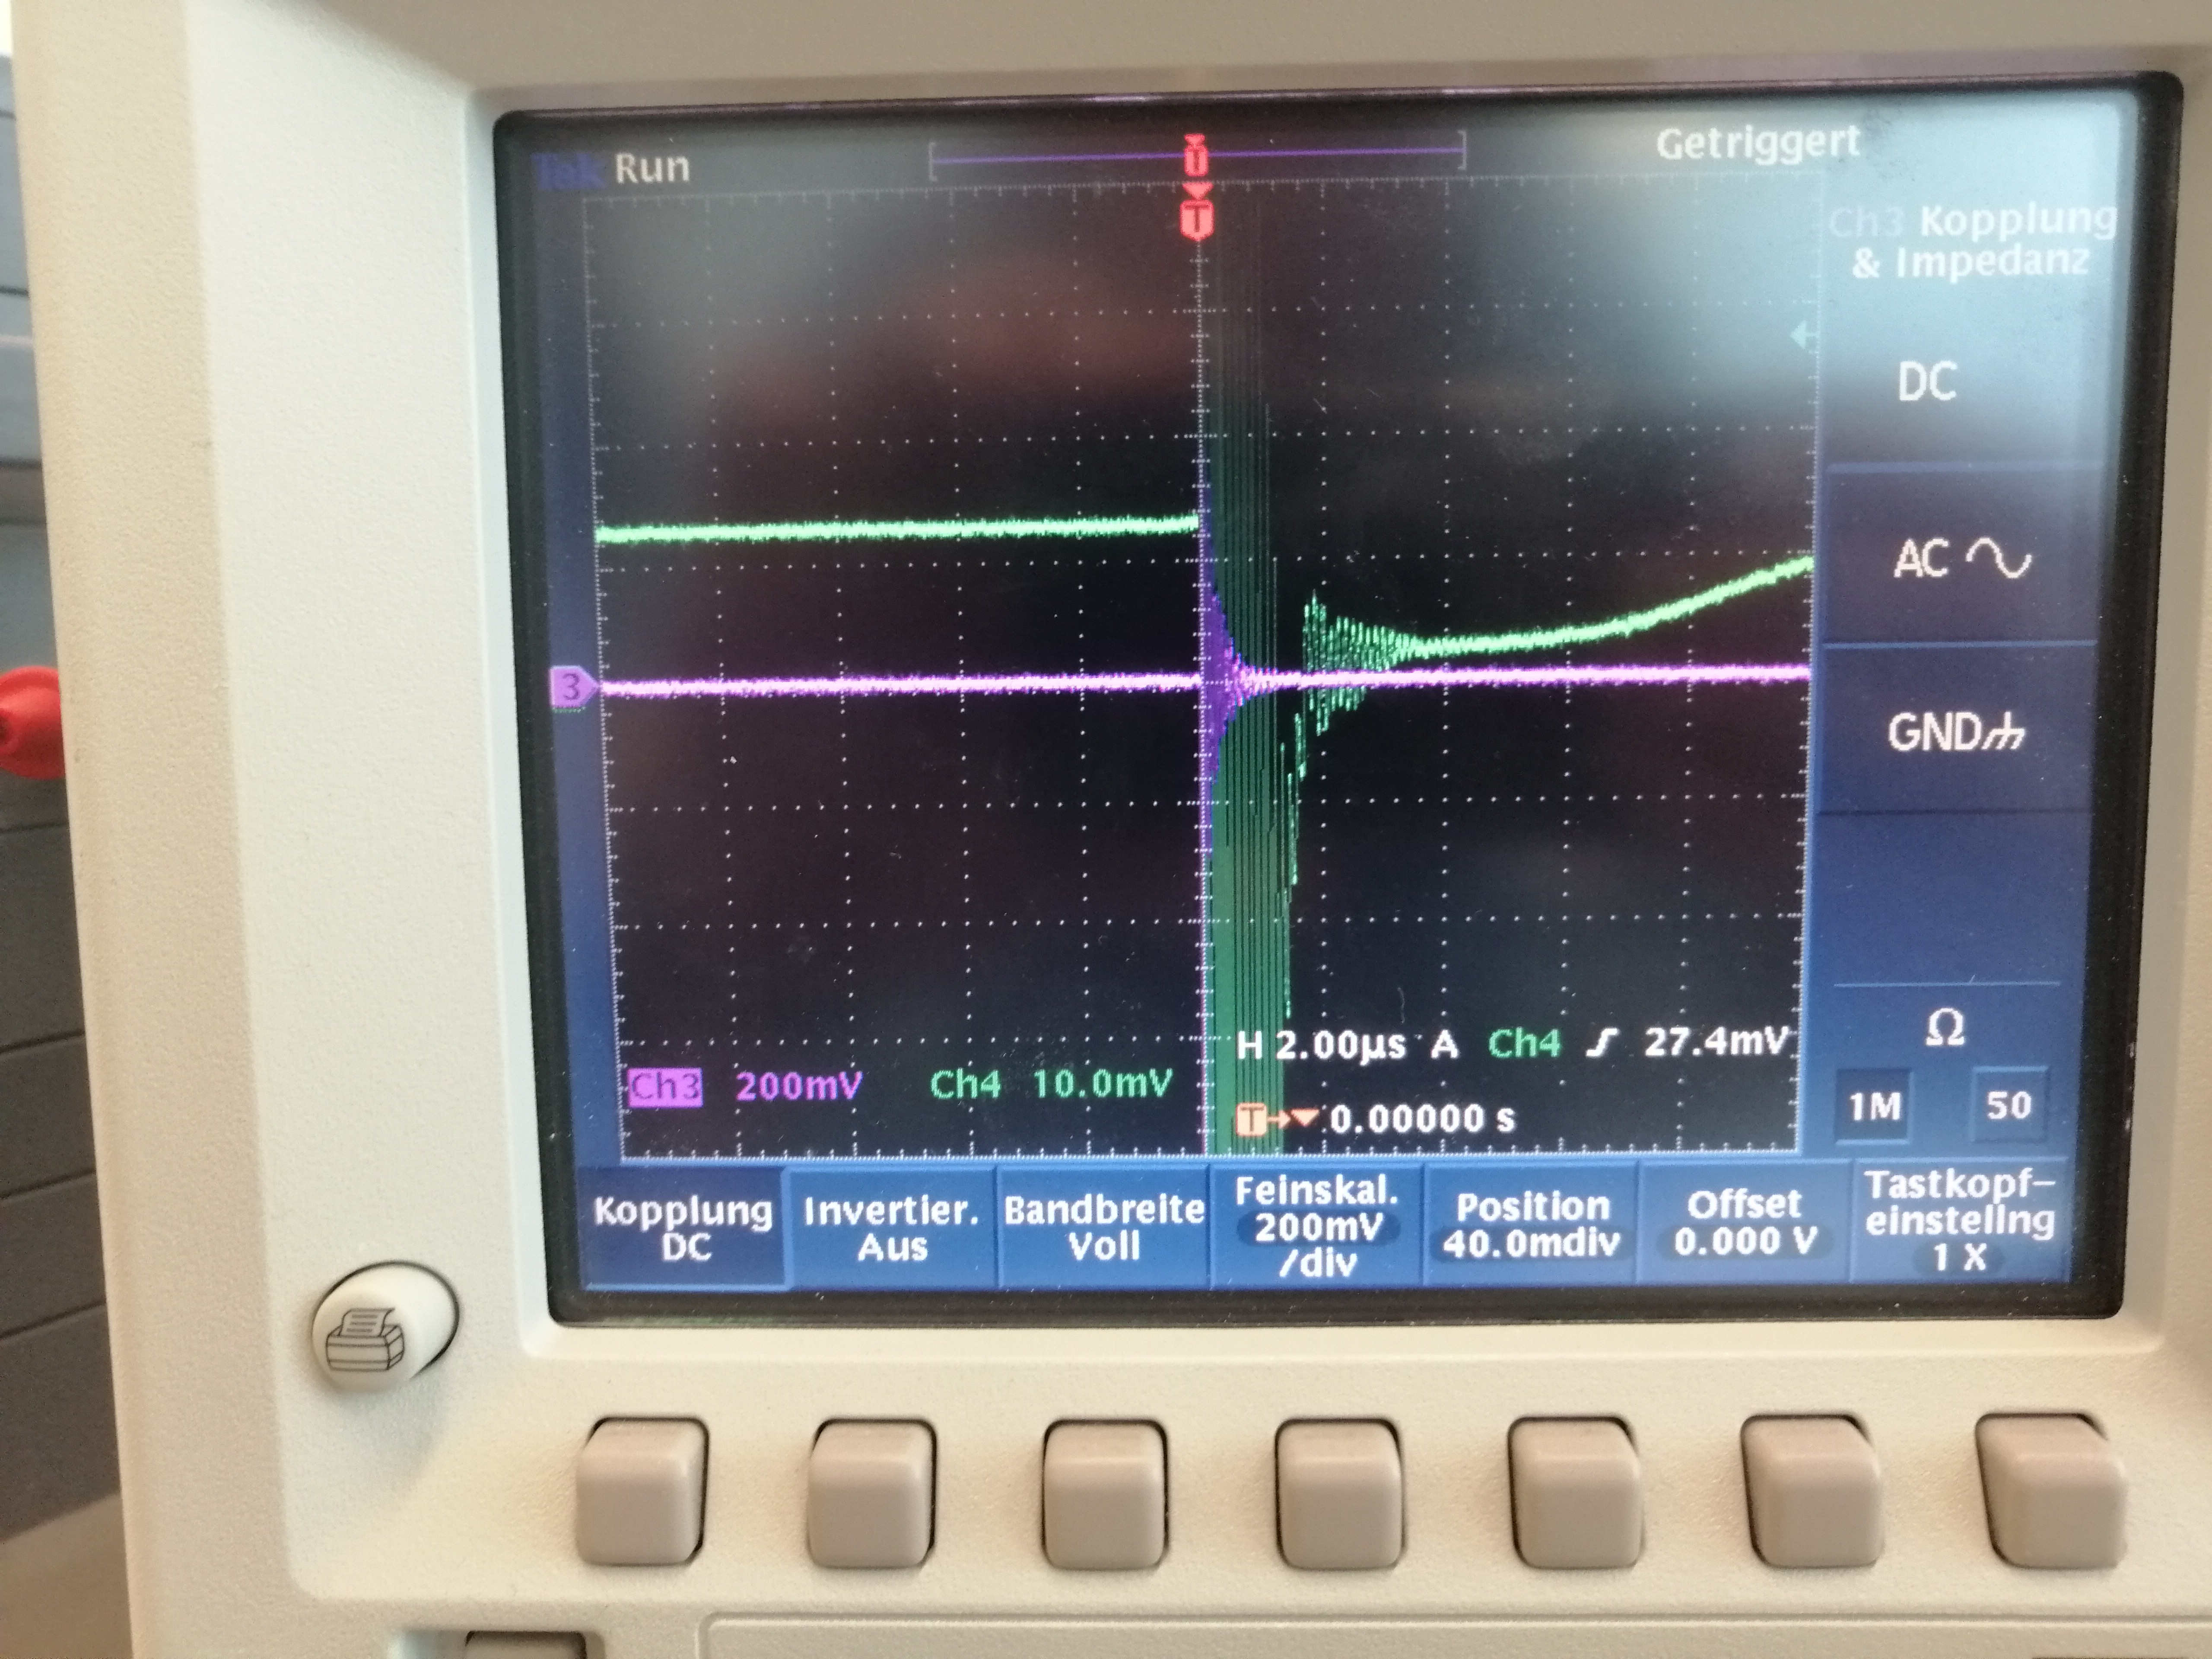
\includegraphics[angle=0,width=0.75\textwidth]{graphics/BurstE2.jpg}
\captionof{figure}{Signal- und Burst-Messung.}
\label{fig:BurstE2}
\end{minipage}
In Abbildung \ref{fig:BurstE2} sind das Signal (Grün) und der Burst (Lila) gegenübergestellt und auf die Flanke hineingezoomt. Man kann leicht erkennen, dass es durch den Burst zu einem Fehler kommt, welcher sich wieder einpendelt.\\
[0.25cm]
\begin{tabular}{|l|l|l|p{5cm}|}
\hline 
\rule[-1ex]{0pt}{2.5ex} Prüfspannung & Prüflevel & Prüfdauer pro Polarität & Auswirkung \\ 
\hline 
\rule[-1ex]{0pt}{2.5ex} 500 V & 1 & 60 s & Verlust der Messfähigkeit bei aktivem Burst. Wieder funktionsfähig unmittelbar nach dem Burst. \\ 
\hline 
\rule[-1ex]{0pt}{2.5ex} 1000 V & 2 & 60 s & Verlust der Messfähigkeit bei aktivem Burst. Wieder funktionsfähig unmittelbar nach dem Burst. \\ 
\hline 
\rule[-1ex]{0pt}{2.5ex} 2000 V & 3 & 60 s & Verlust der Messfähigkeit bei aktivem Burst. Wieder funktionsfähig unmittelbar nach dem Burst. \\ 
\hline 
\rule[-1ex]{0pt}{2.5ex} 4000 V & 4 & 60 s & Verlust der Messfähigkeit bei aktivem Burst. Wieder funktionsfähig unmittelbar nach dem Burst. \\ 
\hline 
\end{tabular} 
\captionof{table}{Prüfungsergebnis Burst-Tests.}
\label{tab:BurstErgebnis}
\vspace*{0.25cm}
Tabelle \ref{tab:BurstErgebnis} listet die Ergebnisse der Burst-Normprogramme auf. Es ist zu erkennen, dass bei jedem Burst-Test die gleichen Auswirkungen zu sehen waren. Die Gesamtauswertung der Tests wird in einem separaten Kapitel (Kapitel \ref{sec:Auswertung}) behandelt.\\

